\documentclass[12pt]{article}
%\usepackage[document]{ragged2e}
\usepackage{array, amssymb, amsthm, linguex, enumerate, amsmath, physics, enumitem, xcolor, graphicx, xparse}
\let\fg\undefined %remove linguex/siunitx naming clash
\usepackage[english]{babel}
\usepackage[letterpaper,top=2cm,bottom=2cm,left=3cm,right=3cm,marginparwidth=1.75cm]{geometry}
\usepackage[colorlinks=true, allcolors=blue]{hyperref}
\usepackage[group-separator={,}]{siunitx} %\num{12345} -> "12,345"
\usepackage{fancyhdr}
\usepackage{notomath}
\usepackage[T1]{fontenc}
\usepackage{multicol}
\usepackage{mathtools}

%Number sets
\newcommand{\R}{\mathbb{R}}
\newcommand{\C}{\mathbb{C}}
\newcommand{\N}{\mathbb{N}}
\newcommand{\F}{\mathbb{F}}
\renewcommand{\Re}{\operatorname{Re}}
\renewcommand{\Im}{\operatorname{Im}}
\renewcommand{\L}[1]{\mathcal{L}\left({#1}\right)} %Linear Map

\newcommand{\pmp}{\,\pm\,} %add small extra space to \pm

\NewDocumentCommand{\ceil}{ s m }{% ceiling brackets
    \IfBooleanTF{#1}%
    {\lceil #2 \rceil}% starred: no-autosizing
    {\left\lceil #2 \right\rceil}% unstarred: autosizing
}

\NewDocumentCommand{\ceiling}{ s m }{% ceiling brackets
    \IfBooleanTF{#1}%
    {\lceil #2 \rceil}% starred: no-autosizing
    {\left\lceil #2 \right\rceil}% unstarred: autosizing
}

\NewDocumentCommand{\floor}{ s m }{% floor brackets
    \IfBooleanTF{#1}%
    {\lfloor #2 \rfloor}% starred: no-autosizing
    {\left\lfloor #2 \right\rfloor}% unstarred: autosizing
}

\NewDocumentCommand{\pars}{ s m }{% parenthesis
    \IfBooleanTF{#1}%
    {( #2 ) }% starred: no-autosizing
    {\left( #2 \right) }% unstarred: autosizing
}

\NewDocumentCommand{\inner}{ s m }{% inner product
    \IfBooleanTF{#1}%
    {\langle #2 \rangle}% starred: no-autosizing
    {\left\langle #2 \right\rangle}% unstarred: autosizing
}

\NewDocumentCommand{\innerconj}{ s m }{% inner product
    \IfBooleanTF{#1}%
    {\overline{\langle #2 \rangle}}% starred: no-autosizing
    {\overline{\left\langle #2 \right\rangle}}% unstarred: autosizing
}

\NewDocumentCommand{\brac}{ s m }{% brackets
    \IfBooleanTF{#1}%
    {[#2] }% starred: no-autosizing
    {\left[ #2 \right] }% unstarred: autosizing
}

%default latex bracket size naming
\newcommand{\biggbrac}[1]{\bigg[ {#1} \bigg] }
\newcommand{\bigbrac}[1]{\big[ {#1} \big] }
\newcommand{\Bigbrac}[1]{\Big[ {#1} \Big] }


\RenewDocumentCommand{\over}{ s m }{% fraction 1/arg
    \IfBooleanTF{#1}%
    {\dfrac{1}{#2}}% starred: dfrac
    {\frac{1}{#2}}% unstarred: normal frac
}

\NewDocumentCommand{\pover}{ s m }{% parenthesis around fraction (1/arg)
    \IfBooleanTF{#1}%
    {\left(\dfrac{1}{#2}\right)}% starred: dfrac
    {\left(\frac{1}{#2}\right)}% unstarred: normal frac
}

\NewDocumentCommand{\pfrac}{ s m m}{% parenthesis around fraction (arg1/arg2)
    \IfBooleanTF{#1}%
    {\left( \dfrac{{#2}}{{#3}} \right)}% starred: dfrac
    {\left( \frac{{#2}}{{#3}} \right)}% unstarred: normal frac
}


\newcommand{\Xbar}{\bar{X}}
\newcommand{\Ybar}{\bar{Y}}
\newcommand{\xbar}{\bar{x}}
\newcommand{\ybar}{\bar{y}}

\newcommand{\symint}[1]{\int_{- #1}^{#1}}

\newcommand{\limn}{\lim_{n\to\infty}}

\newcommand{\sumn}[1]{\sum_{n=#1}^{\infty}}

\newcommand{\nptl}{\frac{n \pi t}{L}}
\newcommand{\npt}{n \pi t}
\newcommand{\npto}[1]{\frac{n \pi t}{#1}}

\newcommand{\npxl}{\frac{n \pi x}{L}}
\newcommand{\bnxl}{\frac{\beta_n x}{L}}
\newcommand{\npx}{n \pi x}
\newcommand{\np}{n \pi}
\newcommand{\npxo}[1]{\frac{n \pi x}{#1}}
\newcommand{\onp}[1]{\frac{#1}{n \pi}}
\newcommand{\onps}[1]{\frac{#1}{n^2 \pi^2}}
\newcommand{\onpc}[1]{\frac{#1}{n^3 \pi^3}}
\newcommand{\npo}[1]{\frac{n \pi}{#1}}
\newcommand{\cosp}[1]{\cos \pars{#1}}
\newcommand{\sinp}[1]{\sin \pars{#1}}
\newcommand{\intll}{\int_{-L}^{L}}
\newcommand{\intl}{\int_{0}^L}

\newcommand{\gammaDist}[2]{\operatorname{Gamma} \left( {#1},{#2} \right)} %gamma distribution
\NewDocumentCommand{\normalDist}{s g g}{ %normal distibution
    \IfBooleanTF{#1} { % starred, no autosizing parenthesis
      \IfNoValueTF{#2}{
          N (\mu,\, \sigma^2 ) %\normalDist* "default" normal distribution N(\mu, \sigma^2)
        } {
            \IfNoValueTF{#3}{N (#2)}{} %\normalDist{arg} --> N(arg)
        }
      \IfNoValueTF{#3}{}{N ( #2, #3 )}  %\normalDist*{arg1}{arg2} --> N(arg1,arg2)
    }  % else (unstarred) autosize parenthesis
    {
        \IfNoValueTF{#2}{
            N \left(\mu,\, \sigma^2 \right) %\normalDist "default" normal distribution N(\mu, \sigma^2)
        } {
            \IfNoValueTF{#3}{N \left(#2\right)}{} %\normalDist{arg} --> N(arg)
        }
        \IfNoValueTF{#3}{}{N \left( #2, #3 \right)} %\normalDist{arg1}{arg2} --> N(arg1,arg2)
    }
}



%colors
\definecolor{ggreen}{RGB}{0, 127, 0}
\definecolor{dgray}{RGB}{63,63,63}
\definecolor{neonorange}{RGB}{255,47,0}
\definecolor{mygray}{rgb}{0.5,0.5,0.5}
\definecolor{eblue}{RGB}{0,74,127}
\newcommand{\red}[1]{\color{red}{#1}\color{black}}
\newcommand{\green}[1]{\color{ggreen}{#1}\color{black}}
\newcommand{\blue}[1]{\color{blue}{#1}\color{black}}
\newcommand{\setRed}{\color{red}}
\newcommand{\setBlack}{\color{black}}
\newcommand{\setBlue}{\color{blue}}
\newcommand{\setGreen}{\color{ggreen}}

\newcommand{\coshp}[1]{\cosh \pars{#1}}
\newcommand{\sinhp}[1]{\sinh \pars{#1}}
\newcommand{\cunt}{\frac{c n \pi t}{L}}
\newcommand{\absl}{\abs{\lambda}}
\newcommand{\rabsl}{\sqrt{\abs{\lambda}}}
\newcommand{\qiffq}{\quad\iff\quad}
\newcommand{\thru}[1]{{#1}_1, \dots, {#1}_n}
\newcommand{\sumThru}[1]{{#1}_1 + \cdots + {#1}_n}
\newcommand{\yn}{Y_1, \dots, Y_n} % Y_1, ..., Y_n
\newcommand{\xn}{X_1, \dots, X_n} % Y_1, ..., Y_n

%hats and tildes
\newcommand{\that}{\widehat{\theta}} % theta hat
\newcommand{\phat}{\widehat{p}} % p hat
\newcommand{\qhat}{\widehat{q}} % p hat
\newcommand{\psihat}{\widehat{\psi}} % psi hat
\newcommand{\Psihat}{\widehat{\Psi}} % Psi hat
\newcommand{\ptilde}{\widetilde{p}} % psi tilde
\newcommand{\Psitil}{\widetilde{\Psi}} % Psi tilde
\newcommand{\betah}{\widehat{\beta}} % beta hat

%2x2 matrix shortcuts
\newcommand{\detx}[4]{\begin{vmatrix}{#1} & {#2}\\{#3}&{#4}\end{vmatrix}} % 2x2 determinant
\newcommand{\dety}[9]{\begin{vmatrix}{#1} & {#2} & {#3} \\{#4}&{#5}&{#6}\\ {#7} & {#8} & {#9}\end{vmatrix}} % 3x3 determinant
\newcommand{\bmaty}[9]{\begin{bmatrix}{#1} & {#2} & {#3} \\{#4}&{#5}&{#6}\\ {#7} & {#8} & {#9}\end{bmatrix}} % 3x3 matrix
\newcommand{\bmat}[4]{\begin{bmatrix}{#1} & {#2}\\{#3}&{#4}\end{bmatrix}} % 2x2 matrix brackets
\renewcommand{\pmat}[4]{\begin{pmatrix}{#1} & {#2}\\{#3}&{#4}\end{pmatrix}} % 2x2 matrix parenthesis

%remove any enumerate/itemize indent temporarily
\makeatletter   %% <- make @ usable in macro names
\newcommand*\notab[1]{%
  \begingroup   %% <- limit scope of the following changes
    \par        %% <- start a new paragraph
    \@totalleftmargin=0pt \linewidth=\columnwidth
    %% ^^ let other commands know that the margins have been reset
    \parshape 0
    %% ^^ reset the margins
    #1\par      %% <- insert #1 and end this paragraph
  \endgroup
}
\makeatother    %% <- revert @


\newcommand{\dimrange}[1]{\operatorname{dim}\operatorname{range}{#1}} % dimrange
\newcommand{\dimnull}[1]{\operatorname{dim}\operatorname{null}{#1}} % dimnull
\newcommand{\range}[1]{\operatorname{range}{#1}} %range
\newcommand{\nullspace}{\operatorname{null}} %null

% polynomial notation
\NewDocumentCommand{\poly}{ s g g }{%
    \IfBooleanTF{#1} {
        \IfNoValueTF{#2} {
            \mathcal{P}(\mathbb{R})
        } {
            \mathcal{P}_{#2}(\mathbb{R})
        }
    } {
        \IfNoValueTF{#3} {
            {\mathcal{P}(#2)}
        } { %else
            {\mathcal{P}_{#2}(#3)}
        }
    }
}

\NewDocumentCommand{\bias}{ s m }{% bias(arg)
    \IfBooleanTF{#1}%
    {\operatorname{bias}(#2)}% starred: no autosizing
    {\operatorname{bias}\left(#2\right)}% unstarred: autosizing
}

\NewDocumentCommand{\MSE}{ s m }{% MSE(arg)
    \IfBooleanTF{#1}%
    {\operatorname{MSE}(#2)}% starred: no autosizing
    {\operatorname{MSE}\left(#2\right)}% unstarred: autosizing
}

\NewDocumentCommand{\Var}{ s m }{% variance with parenthesis V(arg)
    \IfBooleanTF{#1}%
    {\operatorname{Var}(#2)}% starred: no autosizing
    {\operatorname{Var}\left(#2\right)}% unstarred: autosizing
}

\NewDocumentCommand{\Varb}{ s m }{% variance with brackets V[arg]
    \IfBooleanTF{#1}%
    {\operatorname{Var}[\,#2\,]}% starred: no autosizing
    {\operatorname{Var}\left[\,#2\,\right]}% unstarred: has autosizing
}

\NewDocumentCommand{\Vb}{ s m }{% another renaming of variance with brackets V[arg]
    \IfBooleanTF{#1}%
    {\operatorname{Var}[\,#2\,]}% starred: no autosizing
    {\operatorname{Var}\left[\,#2\,\right]}% unstarred: has autosizing
}

\NewDocumentCommand{\E}{ s m }{% expectation with parenthesis E(arg)
    \IfBooleanTF{#1}%
    {\operatorname{E}(#2)}% starred: no autosizing
    {\operatorname{E}\left(#2\right)}% unstarred: has autosizing
}

\NewDocumentCommand{\Eb}{ s m }{% expectation with brackets E[arg]
    \IfBooleanTF{#1}%
    {\operatorname{E}[#2]}% starred: no autosizing
    {\operatorname{E}\left[#2\right]}% unstarred: has autosizing
}

\RenewDocumentCommand{\P}{ s m }{% probability with parenthesis Pr(arg)
    \IfBooleanTF{#1}%
    {\Pr (#2) }% starred: no autosizing
    {\Pr \left( #2 \right) }% unstarred: has autosizing
}

\NewDocumentCommand{\prob}{ s m }{% probability with parenthesis Pr(arg)
    \IfBooleanTF{#1}%
    {\Pr (#2) }% starred: no autosizing
    {\Pr \left( #2 \right) }% unstarred: has autosizing
}

\NewDocumentCommand{\eff}{ s m }{% efficiency with parenthesis eff(arg)
    \IfBooleanTF{#1}%
    {\operatorname{eff}(#2)}% starred: no autosizing
    {\operatorname{eff}\left(#2\right)}% unstarred: has autosizing
}

%vertical vector of up to 8 elements
\NewDocumentCommand\vvec{s m g g g g g g g}{%
    \IfBooleanTF{#1} {
        \begin{bmatrix}% if starred use brackets
            \IfNoValueTF{#2}{}{#2}
            \IfNoValueTF{#3}{}{\\#3}
            \IfNoValueTF{#4}{}{\\#4}
            \IfNoValueTF{#5}{}{\\#5}
            \IfNoValueTF{#6}{}{\\#6}
            \IfNoValueTF{#7}{}{\\#7}
            \IfNoValueTF{#8}{}{\\#8}
        \end{bmatrix}
    }  % else (unstarred) use parethesis
    {
        \begin{pmatrix}%
            \IfNoValueTF{#2}{}{#2}
            \IfNoValueTF{#3}{}{\\#3}
            \IfNoValueTF{#4}{}{\\#4}
            \IfNoValueTF{#5}{}{\\#5}
            \IfNoValueTF{#6}{}{\\#6}
            \IfNoValueTF{#7}{}{\\#7}
            \IfNoValueTF{#8}{}{\\#8}
        \end{pmatrix}
    }
}
\def\Cov{\operatorname{Cov}} %Covariance
\def\df{\text{df}} %degrees of freedom
\def\ARMA{\operatorname{ARMA}}
\def\AR{\operatorname{AR}}
\def\MA{\operatorname{MA}}
\def\SARMA{\operatorname{ARMA}}
\def\SAR{\operatorname{SAR}}
\def\SMA{\operatorname{SMA}}
\def\ACF{\operatorname{SACF}}
\def\PACF{\operatorname{PACF}}
\def\ARIMA{\operatorname{ARIMA}}
\def\SARIMA{\operatorname{SARIMA}}
\NewDocumentCommand{\example}{ s g }{% Example header
    \IfBooleanTF{#1}%
    {\vspace{0.1in}}% starred: 0.1in
    {\vspace{0.2in}}% unstarred: 0.2in
    \IfNoValueTF{#2} {\noindent\textbf{\color{eblue} Example: }}{\noindent\textbf{\color{eblue} Example (#2): }}
}
\NewDocumentCommand{\disc}{ s }{% Discussion header
    \IfBooleanTF{#1}%
    {\vspace{0.1in}\noindent\textbf{Discussion: } }% starred: 0.1in
    {\vspace{0.2in}\noindent\textbf{Discussion: } }% unstarred: 0.2in
}
\NewDocumentCommand{\defn}{ s }{% Definition header
    \IfBooleanTF{#1}%
    {\vspace{0.1in}\noindent\textbf{\color{neonorange} Definition: } }% starred: 0.1in
    {\vspace{0.2in}\noindent\textbf{\color{neonorange} Definition: } }% unstarred: 0.2in
}
\NewDocumentCommand{\reason}{ s }{% Reason header
    \IfBooleanTF{#1}%
    {\vspace{0.1in}\noindent\textbf{Reason:} }% starred: 0.1in
    {\vspace{0.2in}\noindent\textbf{Reason:} }% unstarred: 0.2in
}
\NewDocumentCommand{\recall}{ s }{% Recall header
    \IfBooleanTF{#1}%
    {\vspace{0.1in}\noindent\textit{Recall:} }% starred: 0.1in
    {\vspace{0.2in}\noindent\textit{Recall:} }% unstarred: 0.2in
}
\NewDocumentCommand{\remark}{ s }{% Remark header
    \IfBooleanTF{#1}%
    {\vspace{0.1in}\noindent\textit{Remark:} }% starred: 0.1in
    {\vspace{0.2in}\noindent\textit{Remark:} }% unstarred: 0.2in
}

\NewDocumentCommand{\soln}{ s }{% Remark header
    \IfBooleanTF{#1}%
    {\vspace{0.1in}\noindent\textbf{Solution: } }% starred: 0.1in
    {\vspace{0.2in}\noindent\textbf{Solution: } }% unstarred: 0.2in
}
\usepackage{cancel}
\newcommand{\proj}[2]{\operatorname{proj}_{{#1}}{#2}} %projection
\newcommand{\wideand}{\qquad \text{and} \qquad}

\newcommand{\bu}[1]{\textbf{\underline{{#1}}} } %bold underline
\newcommand{\boldit}[1]{\textbf{\textit{{#1}}} } %bold italix

% put actual quotation marks "around something"
\newcommand{\say}[1]{\textquotedblleft{#1}\textquotedblright}

% max{arg} and min{arg}
\renewcommand{\max}[1]{\operatorname{max}\left\{ #1 \right\}}
\renewcommand{\min}[1]{\operatorname{min}\left\{ #1 \right\}}

\newcommand{\Span}[1]{\operatorname{span}\left\{ #1 \right\}}

%Create a new vspace line no indent
\newcommand{\nl}{\vspace{0.1in}\noindent}
\newcommand{\nnl}{\vspace{0.2in}\noindent}
\newcommand{\nnnl}{\vspace{0.3in}\noindent}
\textwidth=7.02in
\hoffset=-.425in

\setcounter{MaxMatrixCols}{20}
\begin{document}
\pagestyle{fancy}
\fancyhf{}
\fancyhead[RO]{Matthew Wilder}
\fancyhead[LO]{MTH 427 - Exam 3}
\fancyfoot[CO]{Page \thepage}

\noindent MTH 427 - Spring 2023
\\Exam 3 - Spring 2023 - MTH 427


\textbf{Conceptual problems}

\textbf{\textit{(Make sure to clearly show your work in order to earn full credit)}}

\section{Exercise 1 (18 points)}
For each of the following $\ARMA$ models, find the roots of the $\AR$ and $\MA$ polynomials,
identify the values of $p$ and $q$ for which they are $\ARMA(p,q)$ (watch out for parameter
redundancy), determine whether they are causal, and determine whether they are invertible.

\begin{enumerate}[label=(\alph*)]
    \item $x_t = -0.3x_{t-1} + w_t - 0.4w_{t-1} - 0.21w_{t-2}$

$$(1+0.3B)x_t = (1-0.4B-0.21B^2)w_t$$
$$\cancel{(1+0.3z)} = \cancel{(1+0.3z)}(1-0.7z)$$
$$\underbrace{1}_{\phi(z)} = \underbrace{1-0.7z}_{\theta(z)}$$
$$x_t = w_t - 0.7w_{t-1} \quad \implies \quad \ARMA(0,1)$$
Since $\phi(z) = 1$ has no roots, the model is causal.\\
Since $\theta(z)$ has one root, $-\frac{10}{3}$, and $\abs{-\frac{10}{3}} > 1$, the model is invertible.
    \item $x_t = 3x_{t-1} + w_t + w_{t-1} - 2 w_{t-2}$

$$(1-3B)x_t = (1+B-2B^2)w_t$$
$$(1-3z) = (1-z)(1+2z)$$
$$\underbrace{1-3z}_{\phi(z)} = \underbrace{(1-z)(1+2z)}_{\theta(z)}$$
$$x_t = 3x_{t-1} + w_t + w_{t-1} - 2 w_{t-2} \quad \implies \quad \ARMA(1,2)$$
Since $\phi(z)$ has root $\frac{1}{3} \leq 1$, the model is not causal.\\
Since $\theta(z)$ has roots 1 and $-\frac12$, and the $\abs{1} \leq 1$, the model is not invertible.
    \item $x_t = 0.5x_{t-1} + 0.5x_{t-2} + w_t - w_{t-1}$

$$(1-0.5B-0.5B^2)x_t = (1-B)w_t$$
$$(1-0.5z-0.5z^2) = (1-z)$$
$$(1+0.5z)\cancel{(1-z)} = \cancel{(1-z)}$$
$$\underbrace{1+0.5z}_{\phi(z)}= \underbrace{1}_{\theta(z)}$$
$$x_t + 0.5x_{t-1} = w_t \quad \implies \quad \ARMA(1,0)$$

\noindent Since $\phi(z)$ only has root $2$ and $2 > 1$, the model is causal.
\\Since $\theta(z)$ has no roots, the model is invertible.
\end{enumerate}

\section{Exercise 2 (8 points)}
Suppose $x_t = w_t - w_{t-4}$, where $w_t$ is a Gaussian white noise $W \sim N (0, \sigma^2_w)$. Find the
mean and the autocovariance function (ACVF) of this series. Show that its autocorrelation
function is nonzero only for lag $h = 4. (h \geq 1)$.

\soln

\nl The mean is zero, $\Eb{x_t} = \Eb{w_t - w_{t-4}} = \Eb{w_t} - \Eb{w_{t-4}} = 0 - 0 = 0$.

\nl The ACVF is 
\begin{align*}
    \Cov(w_t, w_{t+h}) &= \Cov(w_t - w_{t-4},\; w_{t+h} - w_{t+h-4})\\
    &= \underbrace{\Cov(w_t, w_{t+h})}_{\substack{\sigma^2_w \text{ when } h=0\\0 \text{ else}}}
     - \underbrace{\Cov(w_t, w_{t+h-4})}_{\substack{\sigma^2_w \text{ when } h=4\\0 \text{ else}}}
     - \underbrace{\Cov(w_{t-4}, w_{t+h})}_{\text{always 0}}
    + \underbrace{\Cov(w_{t-4}, w_{t+h-4})}_{\substack{\sigma^2_w \text{ when } h=0\\0 \text{ else}}}
\end{align*}

\noindent Since $\Cov(w_a, w_b)$ is zero for $a \neq b$ and $\sigma^2_w$ for $a = b$.

\nl Restricting to $h \geq 1$ means that 
$$\text{ACVF} = \begin{cases}
    - \sigma^2_w & h = 4\\
    0 & h \neq 4
\end{cases} \qquad h \geq 1$$

\nl Therefore the autocorrelation function is only nonzero at lag $h=4$.

\section{Exercise 3 (11 points)}
For those models of \say{Exercise 1} that are causal and invertible, compute the first four coefficients $\pi_0, \pi_1, \pi_2, \pi_3$ in the invertible linear process representation $\pi(B)x_t = \sum_{j=0}^{\infty}\pi_j x_{t-j}$
\\(Hint: set $\sum_{j=0}^{\infty} \pi_j z^j = \frac{\phi(z)}{\theta(z)}$)

\begin{enumerate}[label=(\alph*)]
    \item $x_t = w_t - 0.7w_{t-1} \qquad \qquad \phi(z) = 1 \qquad \theta(z) = 1 - 0.7z$

\begin{align*}
    & \pi_0 + \pi_1 z + \pi_2 z^2 + \pi_3 z^3 + \cdots =\frac{\phi(z)}{\theta(z)} = \frac{1}{1-0.7z}\\
\iff & (1-0.7z)(\pi_0 + \pi_1 z + \pi_2 z^2 + \pi_3 z^3 + \cdots) = 1\\
\iff & \pi_0 + \pi_1 z + \pi_2 z^2 + \pi_3 z^3 + \cdots -0.7 \pi_0z - 0.7 \pi_1 z^2 -0.7 \pi_2 z^3 - 0.7 \pi_3 z^4 + \cdots = 1
\end{align*}

$$\begin{cases}
    \pi_0 = 1 & \implies \pi_0 = 1\\
    \pi_1z -0.7 (1) z = 0 & \implies \pi_1 = 0.7\\
    \pi_2 z^2 - 0.7 (0.7)z^2 = 0 & \implies \pi_2 = 0.49\\
    \pi_3 z^3 - 0.7 (0.49)z^3 = 0 & \implies \pi_3 = 0.343
\end{cases}$$
\setcounter{enumi}{2}
    \item $x_t + 0.5x_{t-1} = w_t \qquad\qquad \phi(z) = 1+0.5z \qquad \theta(z) = 1$


\begin{align*}
    & \pi_0 + \pi_1 z + \pi_2 z^2 + \pi_3 z^3 + \cdots =\frac{\phi(z)}{\theta(z)} = 1+0.5z\\
\iff & \pi_0 + \pi_1 z + \pi_2 z^2 + \pi_3 z^3 + \cdots = 1+0.5z
\end{align*}

$$\begin{cases}
    \pi_0 = 1\\
    \pi_1 = 0.5\\
    \pi_2 = 0\\
    \pi_3 =0
\end{cases}$$
\end{enumerate}

\section{Exercise 4 (14 points)}
Exhibit an equation of the following models. (hint: use you may first use backshift operators,
then expand both sides to obtain an equation in difference form.)
\begin{enumerate}[label=(\alph*)]
    \item $\ARIMA(2,1,1)$.

\nl $p=2,\; d=1, \; q =1$.

\begin{align*}
    & (1 - \phi_1 B - \phi_2 B^2)(1-B)^1 x_t = (1+\theta_1 B)w_t \\
    \iff &\pars{1-(1+\phi_1)B + (\phi_1-\phi_2)B^2 + \phi_2B^3}x_t = (1+\theta_1 B)w_t \\
    \iff & x_t - (1+\phi_1)x_{t-1} + (\phi_1-\phi_2)x_{t-2} + \phi_2 x_{t-3} = w_t + \theta_1 w_{t-1}
\end{align*}
    \item $\ARIMA(1,1,1) \times (0,1,1)_{12}$ or $\SARIMA(1,1,1) \times (0,1,1)_{12}$ (notation from other text books).

\nl $p=1,\; d=1, \; q =1,\; P = 0, \; D=1,\; Q=1,\; S=12$.

Using the model $$\Phi_P(B^s) \phi_p(B)(1-B^s)^D(1-B)^d x_t = \Theta_Q(B^s)\theta_q(B) w_t$$
with 
$$\Phi_P(B^s) = 1, \quad \phi_p(B) = (1-\phi_1B), \quad \Theta_Q(B^s) = (1+\Theta_1 B^{12}), \quad \theta_q(B) = (1+\theta_1 B)$$
gives
$$1(1-\phi_1B)(1-B^{12})^1(1-B)^1x_t =  (1+\Theta_1 B^{12})  (1+\theta_1 B) w_t.$$
Distributing yields 
$$(1-B-B^{12}+B^{13}-\phi_1B + \phi_1 B^2 + \phi_1 B^{13} - \phi_1 B^{14})x_t = (1 + B\theta_1 + \Theta_1 B^{12} + \theta_1 \Theta_1 B^{13})w_t.$$
Writing as a difference equation it becomes
$$x_t - (1+\phi_1)x_{t-1} + \phi_1 x_{t-2} - x_{t-12} + (1+\phi_1)x_{t-13} - \phi_1 x_{t-14} = w_t + \theta_1 w_{t-1} + \Theta_1 w_{t-12} + \theta_1\Theta_1 w_{t-13}.$$
\end{enumerate}

\newpage
\textbf{R Project}
\section{Exercise 5 (8 points)}
Generate $n=100$ observations from $\ARMA(1,1), \AR(1)$ and $\MA(1)$ processes respectively and plot the sample ACF and PACF of each series for $\phi = 0.6, \;\theta = 0.9$. Compare the sample ACFs and PACFs of the generated series with the results given in Table 3.1. (Are these series consistent with the table?)

\notab{\center{
    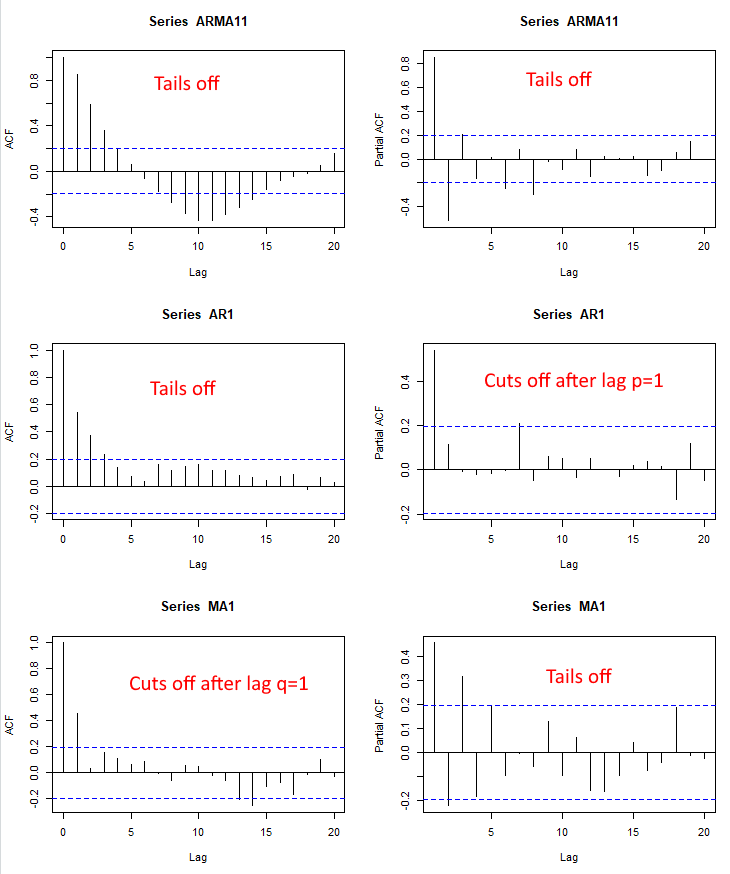
\includegraphics[width=6.25in]{img/5.PNG}
}}

From the following R code:
\begin{verbatim}
    par(mfrow = c(3,2))

    ARMA11=arima.sim(list(order=c(1,0,1), ar=.6, ma=0.9), n=100)
    acf(ARMA11)
    pacf(ARMA11)

    AR1=arima.sim(list(order=c(1,0,0), ar=.6), n=100)
    acf(AR1)
    pacf(AR1)

    MA1=arima.sim(list(order=c(0,0,1), ma=0.9), n=100)
    acf(MA1)
    pacf(MA1)
\end{verbatim}

\nl Compared to the table ({\red{red } text), these results are consistent. When the graph says it cuts off, it \textit{cuts} off. The $\AR(1)$ model looks a little misleading because R isn't labeling the start lag of 1, but tracking back from lag-5 the results hold true. Then all the ones that tail off slowly go towards zero, or oscillate around it.

\newpage
\section{Exercise 6 (13 points)}
Consider the Lake Huron dataset (\say{LakeHuron}) in R or in the package \say{itsmr} as \say{lake}. It consists of $n=98$ observations of annual levels from 1875-1972. Let's investigate if there is evidence of decline in the level of Lake Huron.

\begin{enumerate}[label=(\alph*)]
    \item Plot this series. Plot a sample \textbf{acf} and the sample \textbf{pacf} for this series.

\notab{
    \center{
        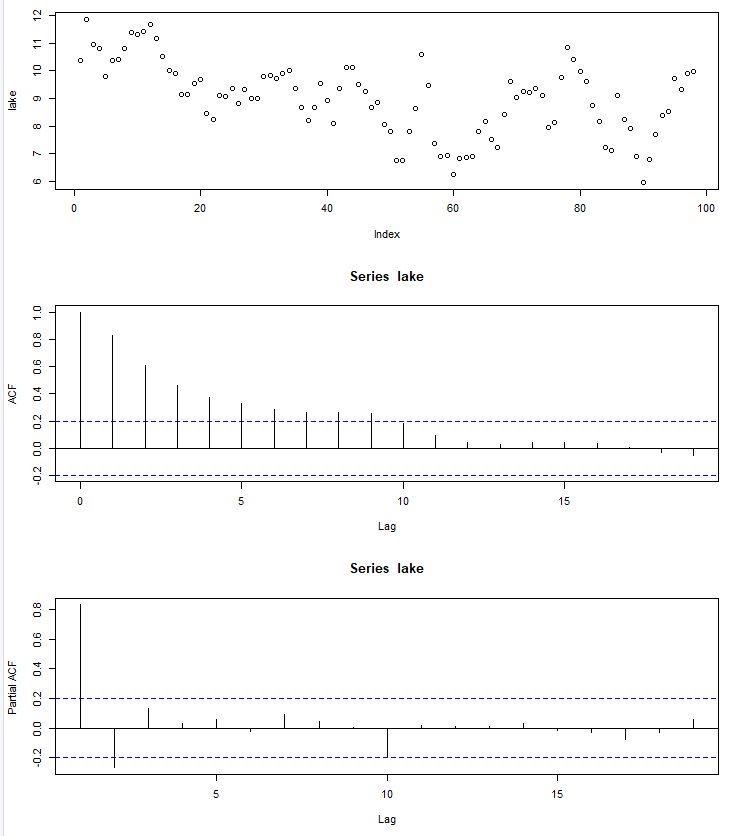
\includegraphics[width=6.75in]{img/6a.PNG}
    }
}

Using the following R code:
\begin{verbatim}
    library(itsmr)
    par(mfrow = c(3,1))
    plot(lake)
    acf(lake)
    pacf(lake)
\end{verbatim}

    \item Based on the \textbf{acf} and \textbf{pacf} in part (a), fit an appropriate ARMA model using \texttt{sarima(p,d,q)} function in R, performing all necessary diagnostics. Comment.

\nl Since the ACF tails off, the model shouldn't be an $\MA(q)$. Since the PACF cuts off after lag $2$, the model could be an $\AR(2)$. This can be fitted with
$$\texttt{sarima(lake,2,0,0, no.constant=TRUE)}.$$
The results of this model are 
\notab{\center{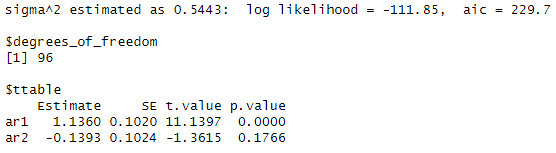
\includegraphics[width=5in]{img/6ar2.PNG}}}
whereby the p-value of one of the coefficients is $0.1766$, which is relatively high, and we want low values. Looking further at the graphs for the model, the ACF of the residuals peaks outside and the Ljung-Box indicates non iid residuals since $\alpha < 0.05$ on some datapoints. The AIC was $229.7$ with $\sigma^2 = 0.5443$, which is fine. 

\notab{\center{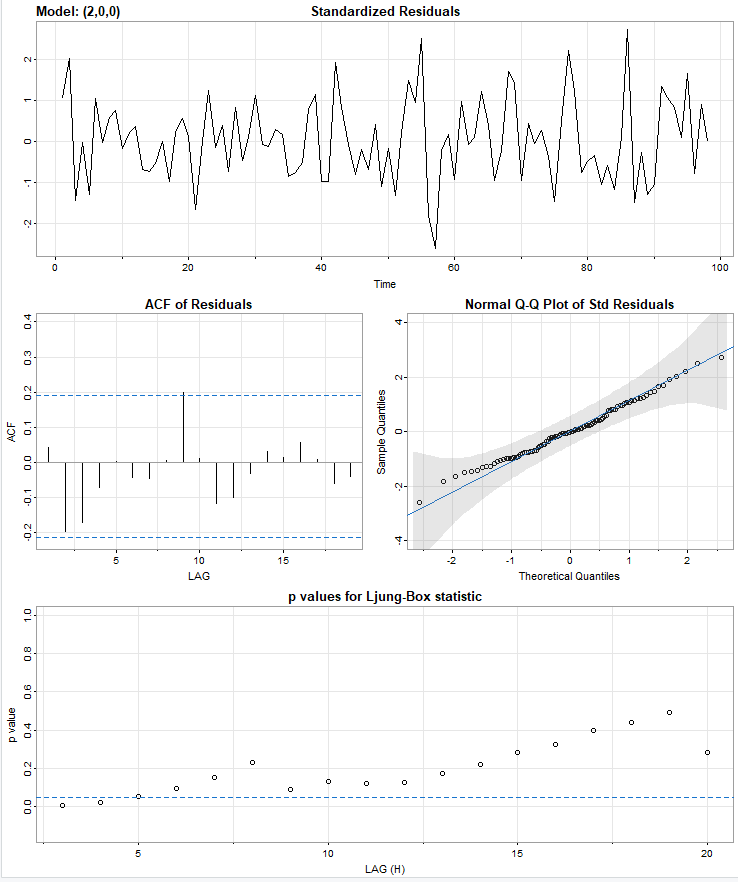
\includegraphics[width=6in]{img/6ar2info.PNG}}}

\nl Moving on to a different model to try and get IID residuals, we can see that the PACF drops even sharper after lag 3, and has almost a large enough drop off after lag 1.

\nl Lag 1 gives good p-values for the coeffient ($p=0$), and has a similar $\sigma^2 = 0.5547$ and AIC of $229.54$. 
\notab{\center{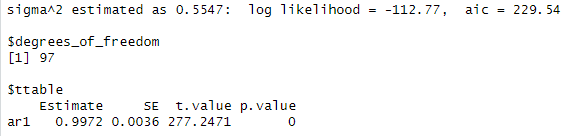
\includegraphics[width=5in]{img/6ar1.PNG}}}

\nl The same problems appear with the diagnostic graphs, though. The Ljung-Box statistic indicates the residuals are not iid and the ACF still spikes. 

\notab{\center{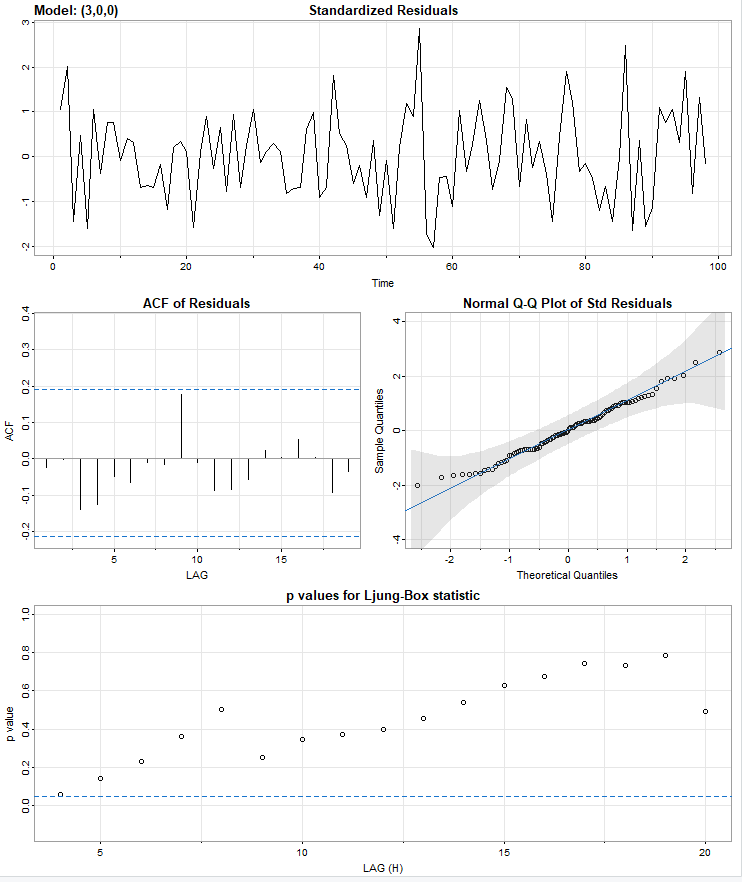
\includegraphics[width=6in]{img/6ar3info.PNG}}}

\nl Finally we settle on Lag 3 because the coefficients are all relatively small with 0.03 being the  max. $\sigma^2 = 0.5183$ is the lowest so far, and same with the AIC of $227.06$. 

\notab{\center{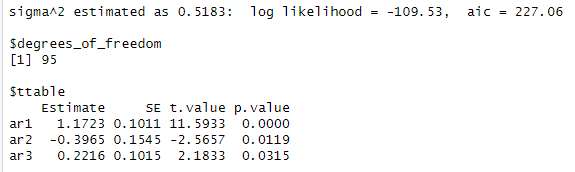
\includegraphics[width=5in]{img/6ar3.PNG}}}

\nl Additionally, the diagnostic graphs are promising too. The Ljung-Box statistic indicates the residuals are iid and the ACF of the residuals has the least spikes of all the tested models. The QQ plot is also a little more normal. For this reason we can conclude that $\AR(3)$ is a good fit for the model. It should be noted that while $\AR(4)$ has a better $\sigma^2$, AIC, and Ljung Box statistic, the p-values of the coefficients are bad, with one of them being 0.80. First differencing also suffered from bad p-values on the coefficients on AR(2) and AR(3), but had lower AICs around 217. Their predictions were flat lines however, so I will ignore those models

\notab{\center{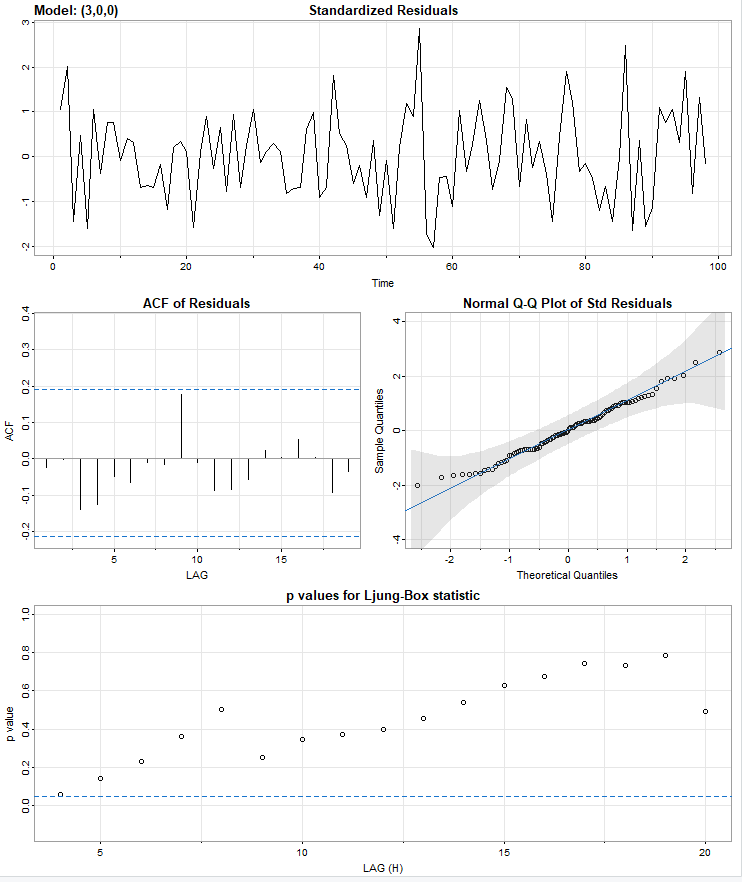
\includegraphics[width=5in]{img/6ar3info.PNG}}}


    \item After deciding on an appropriate model, forecast the data into the future 12 time periods ahead. Make sure to display the plot.

To make the prediction on the selected model, use the following code:
$$\texttt{sarima.for(lake, 12, 3, 0, 0)}$$
\notab{\center{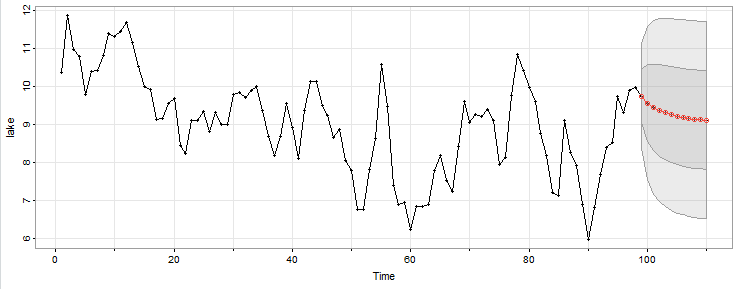
\includegraphics[width=5.5in]{img/6c.PNG}}}
\end{enumerate}

\section{Exercise 7 (28 points)}
Consider the Monthly Airlines Passengers numbers 1949-1960 (airpass) from the package \say{itsmr}, or (AirPassengers) from package \say{astsa} in R.

\begin{enumerate}[label=(\alph*)]
    \item Display the plot of this series and its \textbf{acf} and \textbf{pacf}. Comment on the behavior of this series.
\begin{verbatim}
    par(mfrow = c(3,1))
    plot(airpass)
    acf(airpass)
    pacf(airpass)
\end{verbatim}
\notab{\center{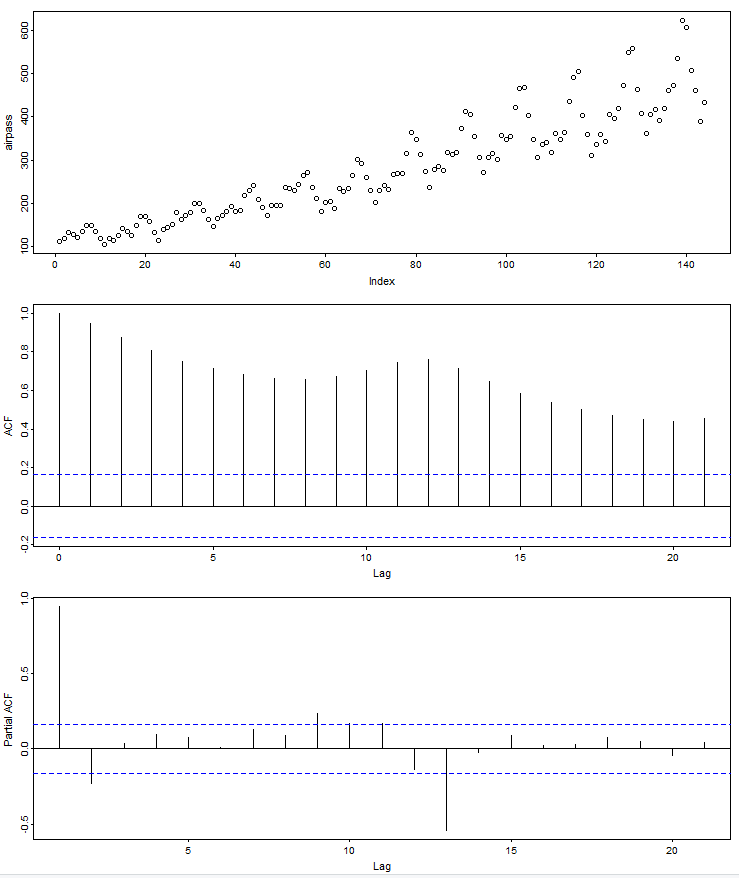
\includegraphics[width=5.5in]{img/7a.PNG}}}

\nl It appears to have a linear increasing trend as well as increasing variance with time. Based on the ACF and PACF plots, an AR(2) seems like a good fit and $\MA(q)$ would be really bad.
    \item Is any transformation necessary? Why?

\nl A log transformation is necessary in order to stabilize the variance. Also detrending the series should be done to remove the linear growth.
    \item Detrend the series by fitting a linear regression of the log-transformed of the series on time $t$. Based on the $R^2$ of this regression fit, can we say that there is a significant trend? Why? (Make sure to display your code and results).

\nl Utilizing the following code: 

\begin{verbatim}
    stableAirpass <- log(airpass)
    fit=lm(stableAirpass~time(stableAirpass))
    par(mfrow=c(2,1))
    plot(as.ts(resid(fit)), main="detrended")
    summary(fit)
    acf(resid(fit),100, main="detrended")
\end{verbatim}
\notab{\center{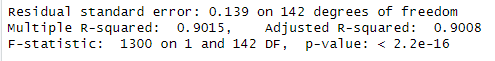
\includegraphics[width=4in]{img/7c.PNG}}}
\notab{\center{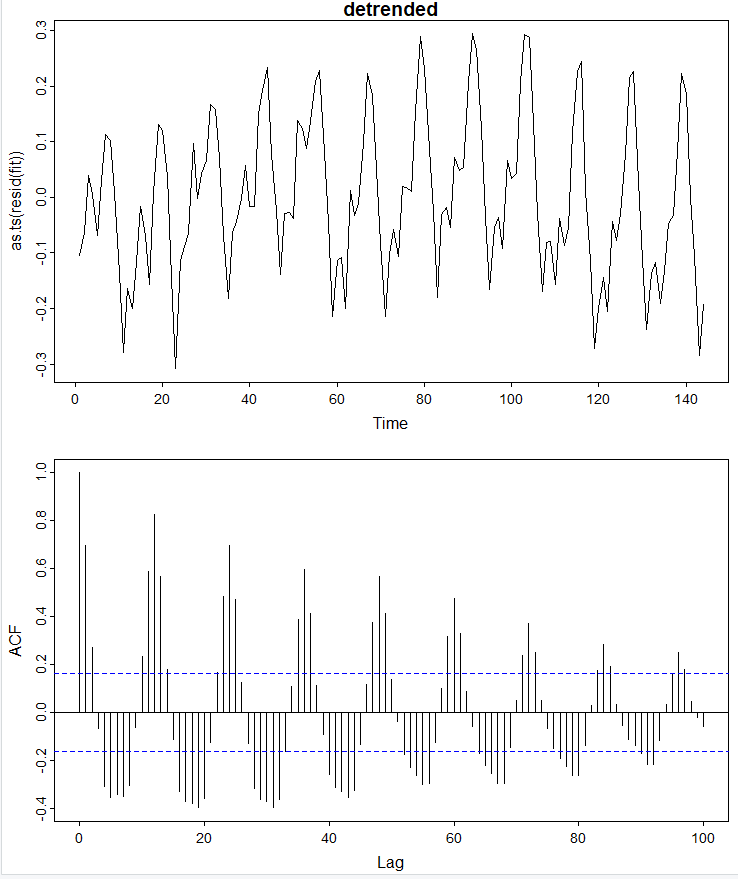
\includegraphics[width=4.5in]{img/7cGraph.PNG}}}

An $R^2 = 0.9$ is a strong linear trend because 90\% of the variance is explained by the model.

\nnl\notab{\textbf{\textit{One can also remove the trend by differencing}}}
    \item Compute the first difference of the log-transformed of the original series. Examine its sample \textbf{acf} plot and compare it with the \textbf{acf} plot of the residuals in part (c). Make sure to display your plots.

\nl Using the following code:
\begin{verbatim}
    diffAirpass <- diff(stableAirpass)
    acf(diffAirpass)
\end{verbatim}

\notab{\center{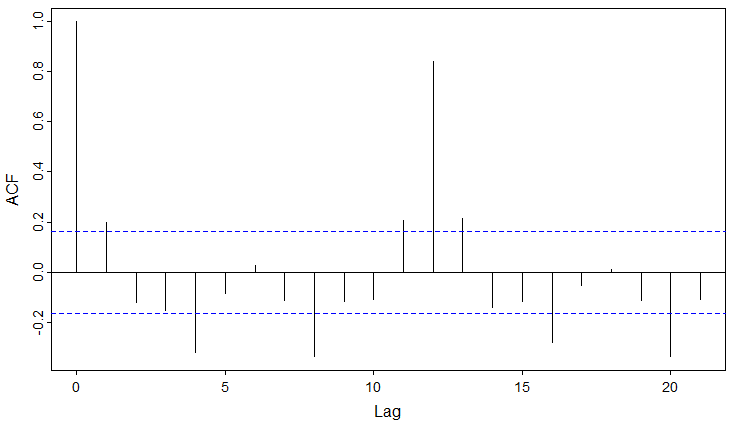
\includegraphics[width=4.5in]{img/7d.PNG}}}

\nl The ACF of the first difference has less data points spiking above the blue dashed line than the linear regression did. This indicates that the residuals of the first difference are less correlated. The first difference stabilizes near zero much faster than the linear regression model, of which slowly decreases in residual size over time. Both graphs still follow a cyclic pattern of period 12.
    \item Is there a strong seasonality in the series? Explain.

\nl There is strong seasonality in the series because of the ACF plots having periodic spikes in the residuals. These occur every 12 datapoints, also known as every year (season). This can also be observed in the detrended data from part (c) whereby it follows a fairly consistent wave pattern with evenly spaced peaks.
    \item Display a sample \textbf{acf} and \textbf{pacf} of the seasonal difference of the differenced series in part (d). \textit{hint: this line of code is given in the text file \say{Rcode time series-hw8...} posted in Canvas for \say{\textbf{unemp}} series}.

\nl The following code was added, using the series assigned in part (d):
$$\texttt{acf2(diff(diffAirpass, 12), 120)}$$
\notab{\center{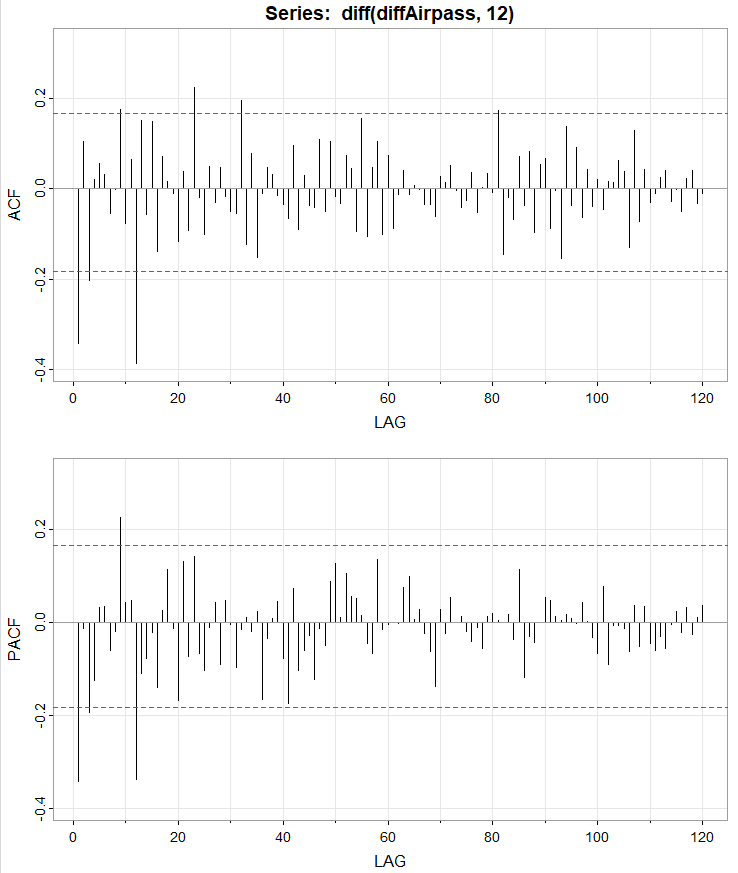
\includegraphics[width=6in]{img/7f.PNG}}}
    \item Based on the \textbf{acf} and \textbf{pacf} in (f), fit an appropriate seasonal ARIMA model to the log transformed Airlines Pasengers series. Make sure to explain why you select that model (model diagnostics).

\nl For the nonseasonal component, both the ACF and PACF cut off after lag 1. This would indicate either $\AR(1), \MA(1),$ or $\ARMA(1,1)$ to be a good starting model. 

\nl For the seasonal component, the ACF and PACF both appear to cut off after lag 1, though its not a perfectly clear seasonal drop, which would also be $\SAR(1), \SMA(1),$ or $\SARMA(1,1)$.

\nl When trying a $\SARIMA(1,1,1) \times (1,1,1)_{12}$ in R, we can look at the coefficents' p-values.
$$\texttt{sarima(stableAirpass, 1,1,1, 1,1,1, 12,no.constant=TRUE)}$$
\notab{\center{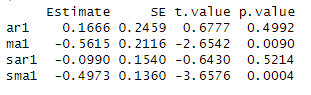
\includegraphics[width=3in]{img/7g.PNG}}}

\nl Dropping the ar1 and sar1 terms due to their large p-values yields a new model
$$\texttt{sarima(stableAirpass, 0,1,1, 0,1,1, 12,no.constant=TRUE)}$$
\notab{\center{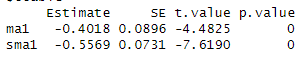
\includegraphics[width=3in]{img/7g2.PNG}}}
With the following diagnostic plots:

\notab{\center{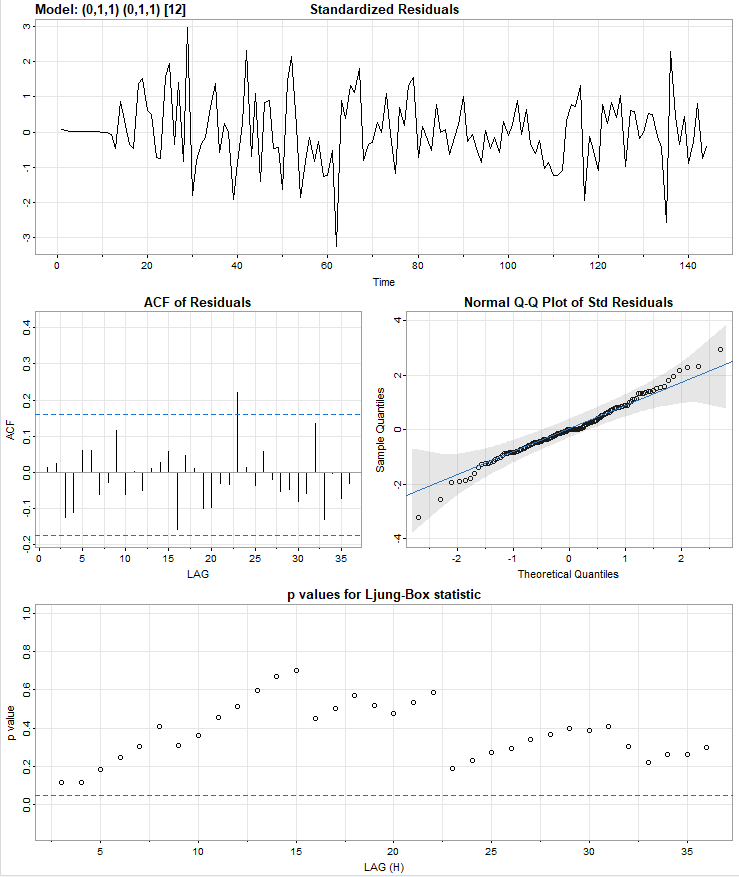
\includegraphics[width=6in]{img/7gPlots.PNG}}}

The Ljung-Box statistic being greater than $\alpha = 0.05$ indicates iid residuals and the QQ plot indicates normally distributed residuals. The R console results also show an estimated $\sigma^2 = 0.0013$ which is very low, along with an AIC of $-483.4$. This seems to be a very good model based on these additional numbers.
    \item Use the estimated model to forecast the next 12 values.

$$\texttt{sarima.for(stableAirpass, n.ahead=12, 0, 1, 1, 0, 1, 1, 12)}$$

\notab{\center{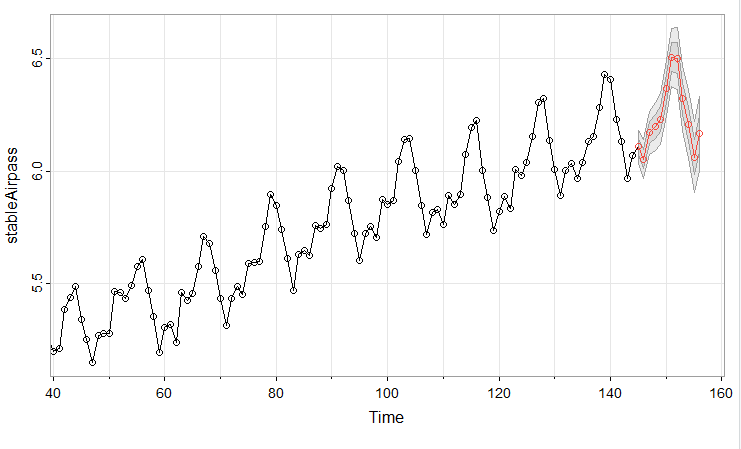
\includegraphics[width=6in]{img/7h.PNG}}}

With a console log for \texttt{\$pred} indicating the following exact values:
\begin{verbatim}
    6.110186
    6.053775
    6.171715
    6.199300
    6.232556
    6.368779
    6.507294
    6.502906
    6.324698
    6.209008
    6.063487
    6.168025
\end{verbatim}
\end{enumerate}


\end{document}
